\section{Chapter 11: Visual Thinking Processes}
\graphicspath{ {pngs/ch11/} }


\secttoc

Foraging for food has much in common with foraging for information.
Both must be done efficiently, often there are large gaps between finding
succulent food or information clusters. There is also a scent indicating where
these may be.

The common bottleneck in visual thinking is our limited working memory
capacities. This is why rapid attention shifts must be made possible.

In this new field, there is still much to invent and improve. As the years
pass, these innovations will become standards for information
professionals; like clay hardening in the kiln.

\begin{mdframed}\begin{multicols}{2}
\subsection{Cognitive System}
We will focus on \textbf{epistemic actions}, simple ones triggered by the user
where rapid transformations change what is presented.

\begin{figure}[H] \centering
    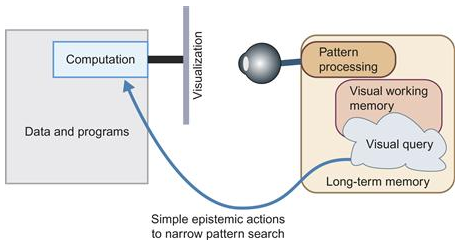
\includegraphics[width=0.8\linewidth]{cognitive_system.png}
    \caption{The system considered in this chapter.}
\end{figure}



\subsection{Memory and Attention}
\begin{compactdesc}
\item[Iconic memory] short-term, holds retinal image for a few hundred ms or
    until replaced, no semantics
\item[Visual working memory (VWM)] holds objects of immediate attention, usually a
    combination of images and semantics from long-term memory
\item[Long-term memory] everyday use, may last a lifetime, tight links to
    working memory
\item[Working memories] separate systems for auditory, visual information;
    also body movements, verbal output. There may be more for cognitive
    instructions and motor control. They are mostly independently.
\item[Visual working memory capacity] position, some abstract shape, color,
    texture are retained from one fixation to the next. Limited to three to
    five simple objects. Example: simple mushroom stem and cap count as two
    objects. Integrated glyphs allow more info to be held.
\item[Change blindness] we don't see the world's complexity and detail at
    the same time! It only seems that way because of our long-term memory
    (provides gist) and details are there when we want them. Experiment: people
    failed to notice when their new partner was swapped mid-conversation.
\item[Spatial information] possible to store up to nine ego-centric
    locations. Separate from retinal locations.
    Can hold three to five moving objects across fixations.
\item[Attention] to hold three to four objects in VWM takes a lot of attention.
    Inattentional blindness is possible: i.e. an unexpected pattern appears
    and test subject doesn't notice it. Attention's selectivity isn't perfect,
    see the Stroop effect.
\item[Object files, coherence fields, gist]
    Object files in Chapter 8. Gist: verbal-propositions recalled by images
    from long-term memory within 100ms.
    Typical locations, general information remembered.

\end{compactdesc}
\end{multicols}\end{mdframed}

\begin{mdframed}\begin{multicols}{2}
\begin{figure}[H] \centering
    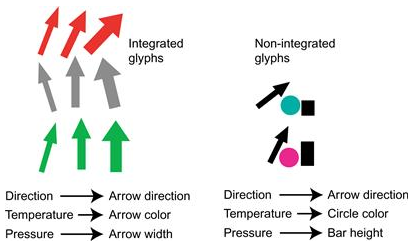
\includegraphics[width=0.6\linewidth]{integrated_glyphs.png}
    \caption{Integrated glyphs allow more information to be held in
    visual working memory.}
\end{figure}
\begin{figure}[H] \centering
    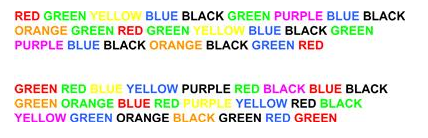
\includegraphics[width=0.8\linewidth]{stroop_effect.png}
    \caption{Stroop effect: the colors of the lower set of words cannot
    be easily spoken in sequence.}

\end{figure}
\end{multicols}\end{mdframed}





\begin{mdframed}\begin{multicols}{2}
\subsection{Long-term memory}
\begin{compactdesc}
\item[Long-term memory] built up over a lifetime. Includes verbal material,
    motor skills, perceptual skills. Not all of it is conscious.
\item[Episodic memory] memories associated with events.
\item[Hippocampus] appears to form long-term memories.
\item[Memory trace theory] memories are traces -- neural pathways made of
    strengthened connections. Explains priming and recognition $>$ recall.
\item[Chunks and concepts] interchangeable terms here. The grouping of
    objects into more complex ones. Expertise = effective high-level
    concepts.
\end{compactdesc}


\subsection{Knowledge formation, creative thinking}
\begin{compactdesc}
\item[Bayesian approach] learning done through repeated exposure, neural
    pathways strengthened.
\item[Physicalist theory] new concepts built on top of old ones. Single
    event learning of new concepts.
\item[Teaching] hill climbing problems can be solved by
    using simulated annealing (controlled randomness, metallurgic term).
    Students saw visualization of red dots bouncing on terrain with local
    min and absolute min. With increased randomness, the dots avoided the
    local min.
\item[Results] students had to solve a similar problem. Finding a path
    through obstacles can be accomplished with similar simulated annealing.
\item[Knowledge transfer] deep learning. (Animations shouldn't be too concrete)
    Formed by a kind of hypothesis-testing mechanism.
\end{compactdesc}

\end{multicols}\end{mdframed}





\begin{mdframed}\begin{multicols}{2}
\subsection{Visualizations and Mental Images}
Diagrams can be built mentally, without external aid.
Properties of mental images:
\begin{compactdesc}
\item[Transitory] fade without cognitive effort
\item[Simple] images only, for most people
\item[Few] items can be imaged
\item[Aggregations] are easy
\item[Operations] can be performed
\item[Logical problems] can be solved with mental images
\item[Same neural] machinery as normal seeing, to some extent
\item[Can be combined with external] imagery. Labeling, additions, deletions,
    other modifications possible. This is a key skill for hypothesis formation.
\end{compactdesc}
\end{multicols}\end{mdframed}





\begin{mdframed}\begin{multicols}{2}
\subsection{Review of Visual Cognitive System Components}
These systems are needed in the construction of visual thinking algorithms.
\begin{compactdesc}
\item[Early visual processing] Motion, color, texture/shape. Two to four
    categories per channel rapidly perceived.
\item[Pattern perception] From contours, areas of texture, color, motion. A few
    simple ones held.
\item[Eye movements] Planned using spatial map of proto-patterns.
    Partial solutions marked in egocentric map.
\item[The intrasaccadic Scanning loop] simple visual shape, processed at
    40msec.
\item[Working memory] three to five items. Attention controls. Part is a rough
    egocentric spatial map.
\item[Mental imagery] our ability to build simple images in mind.
\item[Epistemic Actions] to discover information.
    \begin{compactdesc}
    \item[Attentional switch] 50ms, minimal cognitive effort
    \item[Saccadic eye movement] 150ms, minimal
    \item[Hover query] 1s, medium
    \item[Selection] 2s, medium
    \item[Hypertext jump] 3s, medium
    \item[Zooming] 2s + log change, medium cognitive effort
    \item[Virtual flying] 30s, high
    \item[Virtual walking] 30s, high cognitive effort
    \end{compactdesc}
\item[Visual Queries] hypothesis related to cognitive task. Solved by epistemic
    actions.
\item[Computational Data Mappings] many ways to turn data into pixels. Principle
    of transparency: the user can apply intellect to the task, the tool itself
    seems vanished.
\end{compactdesc}
\end{multicols}\end{mdframed}






\begin{mdframed}\begin{multicols}{2}
\subsection{Visual Thinking Algorithms}



In each, the interplay between information and operations will be considered:
\begin{compactdesc}
\item[Perceptual and cognitive] operation. Anything occuring in the person's
    brain
\item[Displayed information] represented by the visualization.
\item[Epistemic actions] actions designed to seek information
\item[Externalizing] someone saves knowledge by putting it in the world
\item[Computation] parts of the visual thinking algotihm executed by computer
\end{compactdesc}
\end{multicols}\end{mdframed}





\begin{mdframed}
\begin{multicols}{2}
\subsection{Algorithm 1: Visual Queries}
\begin{compactdesc}
\item[Visual query] like a subroutine, components of all visual thinking
    algorithms. A pattern is first cognitively specified, looked for in the
    display, and if found, contributes to the solution of a problem.
\item[Most important] factor is the use of preattentive features for speed.
    Experience also helps a user's speed.
\item[Display environment] a graphic display containing potentially meaningful
visual patterns.
\end{compactdesc}


\midrule\begin{compactenum}
\item Problem components identified that have visual pattern based solutions.
    A visual query is formulated to discriminate between anticipated patterns.
\item Low-level visual system is made sensitive to these patterns. Visual
    scan begun vased on knowledge, display gist, and task.
\item Eye movement made to the next best location based on space
    map, gist, prior location knowledge.
\item Search targets in fixation processed at 40ms per item. Tests are run on
    patterns and objects elicited from proto-patterns and proto-objects.
\item Repeat from 3 as needed. Only a simple description of object and
    pattern components is retained in VWM. Small number of cognitive markers
    placed in spatial map as needed.
\end{compactenum}
\end{multicols}\end{mdframed}





\begin{mdframed}
\begin{multicols}{2}
\subsection{Algorithm 2: Pathfinding}
\begin{compactdesc}
\item[Trip planning] also applies to navigating a network diagram
\item[Visual query construction] city locations are primed, but not kept in
    VWM.
\item[Pattern-finding loop] A path can use up the entire VWM.
    Cognitive labeling helps us reconstruct alternate paths or chunks of a
    path.
\item[Display environment] road map with symbols representing cities, colored
    lines are roads. Can also be node-link diagram.
\end{compactdesc}
\midrule\begin{compactenum}
\item Conduct visual search to find start and end points.
\item Mark these in mental map
\item Find start symbol. Extract patterns relating to particular color that
    trend in right direction. Mark end point symbol of best candidate
    line.
\item Repeat 3 using a new start point until the destination is reached.
\item Push path info into logical proposition store. Little info needed, easy
    to reconstruct.
\item Repeat 3 to find alternative paths, avoiding paths already found.
\end{compactenum}
\end{multicols}\end{mdframed}





\begin{mdframed}
\begin{multicols}{2}
\subsection{Algorithm 3: Hybrid Reasoning: Visual and Mental Imagery}
\begin{compactdesc}
\item[Some reasoning] is well supported by visual operations, thus a mental
    image is helpful.
\item[Display environment] a diagram or other vis representing part of the
    solution to a problem
\end{compactdesc}

\midrule\begin{compactenum}
\item Perceive task-relevant patterns, mentally add semantics.
\item Imagine display modifications.
\item Execute visual queries on the combined internal/external image to solve
    the problem
\end{compactenum}

\end{multicols}\end{mdframed}





\begin{mdframed}
\begin{multicols}{2}
\subsection{Algorithm 4: Design Sketching}
\begin{compactdesc}
\item[Similar to Algorithm 3] now imagined modifications are externalized
\item[Better] it allows more creativity, easier to change and share
\item[Architects] use sketches liberally in their design process
\item[Display environment] Paper and pencil or table computer
\end{compactdesc}
\midrule\begin{compactenum}
\item Imagine some aspect of design
\item Put marks on display to externalize aspects
\item Analytic visual queries to determine if design meets requirements
\item Major flaw? Discard sketch
\item Imagine additions, or reattribute meanings of symbols
\item Visual queries to asses value of imagined additions
\item If acceptable, add marks or erasures
\item Repeat from 5, revising. Repeat from 1, discarding.
\end{compactenum}

\end{multicols}\end{mdframed}





\begin{mdframed}
\begin{multicols}{2}
\subsection{Algorithm 5: Brushing}
\begin{compactdesc}
\item[Brushing] selecting a data object in any view causes it to be
    selected in all other views.
\item[Highlighting] methods MUST support fast search. Try motion if displays
    are crowded.
\item[Display environment] data objects represented in at least two different
    displays
\end{compactdesc}


\midrule\begin{compactenum}
\item Visual query requiring info about a subset of data
\item Select symbols representing relevant subsets
\item Execute visual queries for patterns in the highlighted representation.
    May require info from two or more displays, can be limited by VWM.
\end{compactenum}

\end{multicols}\end{mdframed}





\begin{mdframed}
\begin{multicols}{2}
\subsection{Algorithm 6: Small Pattern Comparisons in a Large Info Space}
\begin{compactdesc}
\item[Multiple windows] Focused details have linked windows.
\item[Zoom interface] comparisons made through rapid scale changes. Better to
    use this if the master pattern fits in VWM.
\item[Rough cost] time = setup + number of comparison queries
\item[Display environment]
\end{compactdesc}

\midrule\begin{compactenum}
\item Epistemic action: navigate to location of the first pattern.
\item Retain subset of pattern in VWM.
\item Epistemic action: navigate to candidate location of a comparison pattern.
\item Compare VWM with candidate. If suitable match found, terminate the
    search. If partial navigate back and forth the two patterns, comparing
    different subsets to each other.
\item If mismatch, repeat from step 1. Mark already-evaluated candidate
    locations.
\end{compactenum}

\end{multicols}\end{mdframed}





\begin{mdframed}
\begin{multicols}{2}
\subsection{Algorithm 7: Degree-of-Relevance Highlighting}
\begin{compactdesc}
\item[Related objects] may become distributed across the display.
\item[Degree of relevance] highlighting: when an object is selected, all related
    objects are highlighted as well.
\item[Useful for] 30 to thousands of objects. Very effective if the ranking
    function can filter highlighted objects to 10 or 20 objects.
\item[Display environment] display containing many symbols linked by complex
    overlapping set of relationships
\end{compactdesc}

\midrule\begin{compactenum}
\item Construct visual query to find a symbol with potentially useful
    information (``scent'').
\item Epistemic: select symbol.
\item Computer highlights all symbols with a high degree of relevance to this
    symbol.
\item Visual pattern query for more information ``scent''
\item If high relevance symbol is found, execute addition epistemic action
    to find more info. Usually shown in another window.

\item Repeat from 1 as needed.
\end{compactenum}
\end{multicols}\end{mdframed}





\begin{mdframed}
\begin{multicols}{2}
\subsection{Algorithm 8: Generalized Fisheye Views}
\begin{compactdesc}
\item[Beneficial] with hierarchical data. Removes clutter by hiding
    irrelevant elements.
\item[Downside] important information is hidden
\item[Degree of relevance] function determines what is shown and what is not
\item[Display environment] a set of symbols representing entities from a
    much larger set. Entities linked by complex overlapping set of
    relationships
\end{compactdesc}

\midrule\begin{compactenum}
\item Visual query to find info accessible via particular symbol. Conduct
    search.
\item Epistemic action: select symbol.
\item Computer displays all symbols representing data above computer relevance
    threshold. Can weigh so that most salient displayed with most detail.
    Irrelevant symbols are hidden.
\item Visual query to find info in updated display.
\item If high relevance symbol is found, execute addition epistemic action
    to find more info. Usually shown in another window.
\item Repeat from 1 as needed, mentally marking locations of visited symbols.
\end{compactenum}

\end{multicols}\end{mdframed}





\begin{mdframed}
\begin{multicols}{2}
\subsection{Algorithm 9: Multidimensional Dynamic Queries with Scatter Plot}
\begin{compactdesc}
\item[Multidimensional discrete data] all entities have the same set of
    attributes.
\item[Dynamic queries] control the entities on the display. These are implemented
    as slide bars for each attribute.
\item[Not just scatter plots] can also apply to parallel coordinates.
\item[Display environment] a scatterplot with symbols representing entities
    drawn from a set of multidimensional discrete data, with a set of
    controls restricting range displayed on each data dimension.
\end{compactdesc}

\midrule\begin{compactenum}
\item Visual query addressable by viewing a subset of discrete data defined
    by a hyperbox is constructed
\item Query is executed.
Is the number of targets small enough for the required perception?
Is the pattern found?
\item If high relevance symbol is found, execute addition epistemic action
    to find more info. Usually shown in another window.
\item Execute an epistemic action to change displayed subset by dragging a
    slider that causes the computer to adjust a range on a data dimension.
\item Repeat from 2 until task is successful or abandoned.
\end{compactenum}

\end{multicols}\end{mdframed}





\begin{mdframed}
\begin{multicols}{2}
\subsection{Algorithm 10: Visual Monitoring Strategies}
\begin{compactdesc}
\item[Supervisory control] a system runs on auto-pilot, with occasional input
    from a human operator. Anomalous patterns need to be perceived and
    corrected.
\item[Typical elements] built to account for operator's visual scanning
    strategies:
    \begin{compactdesc}
    \item[Channels] different ways in which information can be received.
        Channels can be display windows, dials, loudspeakers\dots
    \item[Events] signals occurring
    \item[Expected cost] of missing an event
    \end{compactdesc}
\item[Visual scanning patterns influenced] by minimized eye movements (two
    operators within same effective FOV can help). Also by oversampling of
    channels on which infrequent information appears (fixed by
    operators sampling more frequently than required).
\item[Reliabilty Improved by] occasional visual or auditory reminders: such
    as motion which allows different levels of urgency.
\item[High-stress] situations? Hide or dim unnecessary channels in case of dire
    emergencies.
\item[Display environment] a set of glyphs representing status of various
    system components.
\end{compactdesc}

\midrule\begin{compactenum}
\item Setup a cognitive self-interrupt schedule.
\item When an internal cognitive interrupt occurs, scan display with eye
    movements.
    Test each component for patterns requiring action.
\item If such a pattern is found, take action.
\item Repeat from 2 as needed.
\end{compactenum}

\end{multicols}\end{mdframed}





